\section{Parameter Effects}

The effects of the parameters on the model function are straightforward and can be read directly from the previous section.
In summary, the parameter $p_x$ changes the height of the branches $\B$ and $\D$ at their left border, where a lower $p_x$ means a higher value of the model function at these points.
In the previously defined notation, this is written as $\AL_{\B}^-$.
This notation is defined in \Cref{sec:yunus.param.effects}.
The parameter $p_y$ changes the offset of branches $\A$ and $\C$, so it moves the whole branches in contrast to $p_x$.
A higher $p_y$ means a higher offset and it is written as $\AW_{\A}^+$.

\todo{write about illustrations}

\begin{figure}
    \centering
    \begin{subfigure}{0.4\textwidth}
        \centering
        \includegraphics[width=\textwidth]{60_Final/ParameterEffects/p_x/illustration.png}
        \caption{$p_x$}
        \label{fig:final.param.effects.px}
    \end{subfigure}
    \begin{subfigure}{0.4\textwidth}
        \centering
        \includegraphics[width=\textwidth]{60_Final/ParameterEffects/p_y/illustration.png}
        \caption{$p_y$}
        \label{fig:final.param.effects.py}
    \end{subfigure}
    \caption{Illustration of Parameter Effects}
\end{figure}

\todo{refer to table}
\Cref{sec:yunus.param.effects}

\begin{table}
    \centering
    \begin{tabular}{|c||c|c||c|c|} \hline
        Combined         & $E_0$            & $\chi_0$          & $p_x$        & $p_y$          \\ \hline \hline
        $\AL_{\B}^{-}$   & $\AL_{\B}^{-}$   &                   & $\AL_{\B}^-$ &                \\ \hline
        $\AMi_{\B}^{L-}$ & $\AMi_{\B}^{L-}$ & $-\AMi_{\B}^{+}$  &              &                \\ \hline
        $\AW_{\A}^{+}$   &                  & $\AW_{\A}^{+}$    &              & $\AW_{\A}^{+}$ \\ \hline \hline
        $\AB_{\B\C}^{L}$ &                  & $\AB_{\B\C}^{L}$  &              &                \\ \hline
                         & $\AB_{\A\B}^{R}$ & $-\AB_{\A\B}^{L}$ &              &                \\ \hline
    \end{tabular}
    \caption{Comparison of Parameter Effects}
    \label{tab:final.def.parameters.effects}
\end{table}

